\chapter{はじめに}
\label{first}

これは私が微分方程式の解き方を学んでいく中で「この知識を一度体系的にまとめたい」と思って書いたものです。私の持つ知識の範疇で微分方程式の解き方をできる限り体系的にまとめました。

微分方程式を「解く」作業には大きく分けて2つの種類があります。

\begin{itemize}
    \item 解析的に解く
    \item 数値的に解く
\end{itemize}

「解析的に解く」とはつまり、図\ref{fig:1-analytical}\footnote{ここでは簡単のため任意定数は1として考えています。}のように式変形を使用して解くことを言います。ですが世の中に存在する微分方程式のほとんどは今の人類には解析的に解くことができません。そんな中でも様々な工夫をすることで、「この形の微分方程式なら解ける」ということを増やすことができます。

\begin{figure}[ht!]
  \centering
  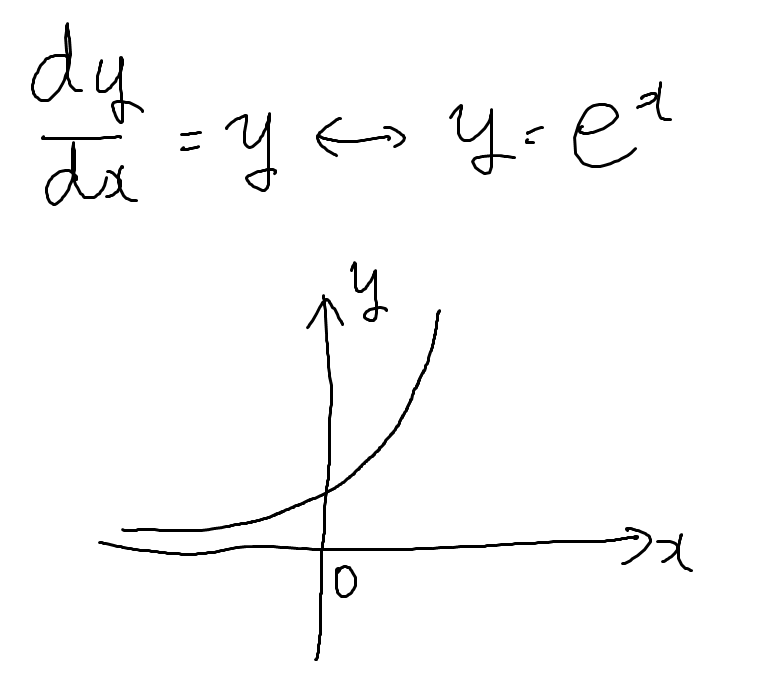
\includegraphics[width=7cm]{img/1-analytical.png}
  \caption{解析的に解く}
  \label{fig:1-analytical}
\end{figure}

「数値的に解く」とは、計算機を用いて微分方程式を近似的に「解く」ことを言います。ここでの「解く」は、何も答えの式が出てくるわけではありません。例えばある$x$における何かの値$y$の数値が、まさに数値として出てくるのです。また、数値的に微分方程式を解いた場合には、求められる解は図\ref{fig:1-numerical}のように離散的(図\ref{fig:1-numerical}ならある決められた値$\Delta x$ごとに$y$が求まります)です。この図についてはこのあと詳しく解説します。

\begin{figure}[ht!]
  \centering
  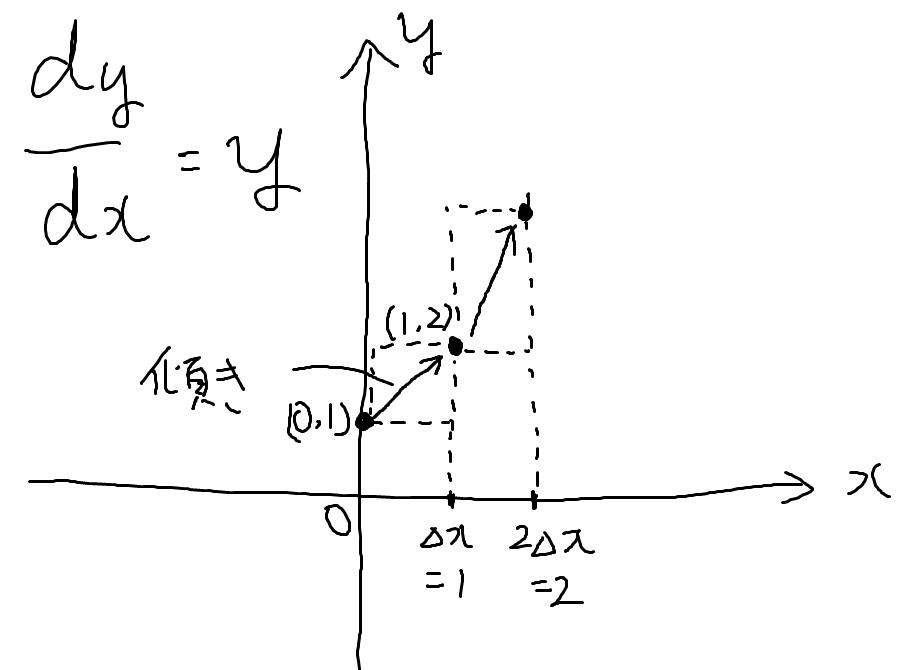
\includegraphics[width=9cm]{img/1-numerical.png}
  \caption{数値的に解く}
  \label{fig:1-numerical}
\end{figure}

本書では微分方程式の解き方についてこの2つの全く異なる方法を解説します。この2つの方法は全く異なるため、便宜上解析的に解く方を先に解説しますが、どちらを先に読んでいただいても構いません。

さて、ここでもう一度図\ref{fig:1-numerical}をご覧ください。これが微分方程式の真髄です。例として出した微分方程式

\begin{eqnarray}
    \frac{\dd y}{\dd x}=y
\end{eqnarray}

\noindent
をもう一度よく睨んでみると……そうです。これは、

\begin{eqnarray}
    (yの傾き)=(yの関数)
\end{eqnarray}

\noindent
という形をしています。「そんなの当たり前じゃないか」と思われる方が大半でしょう。でもよく考えてみてください。ある時点$x$における$y$とそのときの傾きがわかれば、嬉しいことがあります。

\begin{eqnarray}
    y(x+\Delta x)=y(x)+\left.\frac{\dd y}{\dd x}\right|_{x=x}\Delta x
\end{eqnarray}

右辺には既知の値($y$、$\dd y/\dd x$、$\Delta x$)しかありません。そして左辺を見ると、これまでわからなかった$y(x+\Delta x)$が現れています。既知の値を使って未知の値(しかもちょっとだけ$x$が進んだ値)を求める…漸化式みたいですね(実際漸化式の一種だと思います)。

ここで微分方程式の真髄(だと私が思っていること)について一般的な言葉で解説しましょう。

\begin{center}
    「微分方程式はわかっている値を使って「ちょっと先の未来」を知るための方程式である。」
\end{center}

実は解析的に微分方程式を解く場合にはこの真髄が直接役立つことはほぼありません。ですが、「私は今何を解いているのだろう…」と思った時はぜひ思い出してください。「私は未来を知るために微分方程式を解いているのだ」と。

なお、数値的に微分方程式を解くやり方は根本的にこの真髄に従っています。ぜひ覚えておいてください。



\clearpage